\documentclass[12pt,fleqn]{article}\usepackage{../common}
\begin{document}
Ders 5

Bu derste ozel bir ODE turu gorecegiz, bu ODE'lerde sag tarafinda bagimsiz
degisken hic yer almiyor. Bagimsiz degisken $dy/dt = ..$ gibi bir formulde
$t$ degiskenidir, bahsettigimiz turde sag tarafta $t$ iceren bir terim
bulunmaz. Genel olarak

\[ \frac{dy}{dt} = f(y) \]

Tabii bu tur bir denklemde degisken ayirma yontemi kullanmak (bazen, ilk
bakista) kolay. O zaman niye hemen cozmuyoruz? Cevap su ki cozmemize gerek
kalmadan bu tur denklemler hakkinda bazi bilgiler edinmek istiyoruz. Hizli
oldugu icin, bir suru kaliteli bilgi (insight) kazandirdigi icin. Bazen
degisken ayirma da islemeyebilir, ya da denklem hakkinda cok ozel bir soru
sormak istiyoruz ve bu soru icin cozumle ugrasmak istemeyebiliriz.

Grafiksel olarak dusunelim, oncelikle tum isoclines (egimi ayni olan
parcalar) cizimleri duz yataydir. Niye? $dy/dx = f(y)$ turu bir formul her
$x$ (ya da $t$) icin ayni $y$'yi vermek zorundadir, o zaman her $y$ icin (mesela $y_0$
diyelim) egim (slope), yani $dy/dx$ her yerde aynidir, yana dogru duzdur. O
zaman bir $f(y_o)$ icin cizim suna benzer.

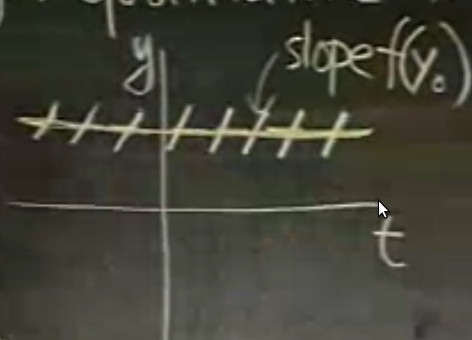
\includegraphics[height=4cm]{5_1.png}

Diger $y$ degerleriyle

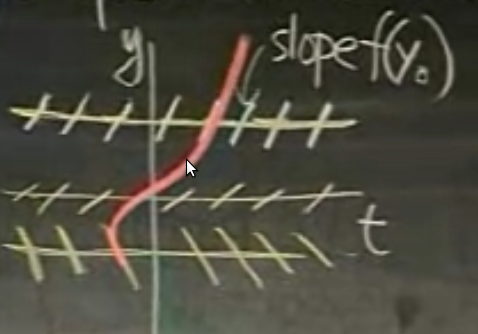
\includegraphics[height=4cm]{5_2.png}

Diger entegral egrileri

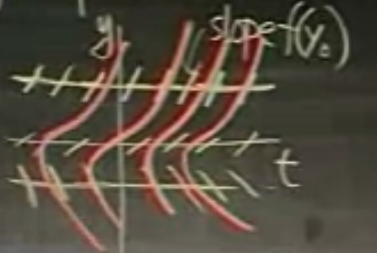
\includegraphics[height=4cm]{5_3.png}

Bu formullerde entegral egrilerinin birisi digerlerinin yana itilmis haline
benzer, yani entegral egileri tasima sirasinda degismez (invariant under
translation) olma ozellige sahiptirler. Birini cizince hepsini gormus
oluruz, digerleri paralel sekilde hemen yandadirlar.

Bilgi nasil elde ederiz? Kritik nokta (critical points) adli kavrami
kullanmamiz lazim.

Kritik Noktalar

Bu noktalar diferansiyelin sifir oldugu $y_0$ noktasidir yani $f(y_o) = 0$.

Adimlar

1. Kritik noktayi bul

2. $f(y)$'yi grafikle, nerede negatif, nerede pozitif bul. Nerede sifir
oldugunu biliyoruz zaten, onun ustunde ve altinda negative ve pozitif
olmasi lazim. Bu niye onemli? Cunku formul unutmayalim ki $dy/dt =
f(y)$. 
Eger $f(y) > 0$ ise o zaman $dy/dt > 0$ demektir yani $y(t)$ artacaktir.

Ornek

$y$ = bankadaki para \\
$r$ = surekli faiz orani

\[ \frac{dy}{dt} = ry \]

Diyelim ki bankada kotu niyetli bir kisi var, paranizi zimmetine
geciriyor. 

$w$ = zimmete gecirme orani

O zaman

\[ \frac{dy}{dt} = ry - w\]

Formulu cozmek kolay, degiskenleri ayir, entegre et. Fakat biz cozmeden,
cozumlerin, $y(t)$'lerin, nasil davrandigina bakalim. ODE bekledigimiz, bu
yazinin konusu olan formda (otonom) cunku sag tarafta $t$ degiskeni
yok. Adimlari takip edelim:

1) Kritik noktayi bulalim

\[ ry - w = 0 \]

\[ y = \frac{w}{r} \]

2) Grafikleyelim

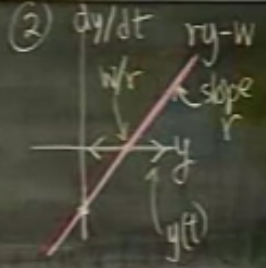
\includegraphics[height=4cm]{5_4.png}

Bu grafikte bizim icin tek onemli sey, nerede $ry-w$ ekseni uzerinde,
nerede onun altinda oldugumuz. Cunku o degerin uzerindeysek $f(y) > 0$, o
zaman $y$ artiyor, digerinde $f(y) < 0$, o zaman $y$ azaliyor. Ortadaki
nokta ise $w/r$ noktasi.

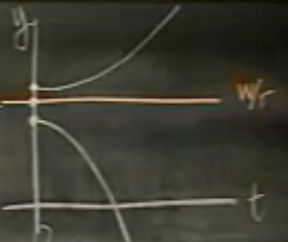
\includegraphics[height=4cm]{5_5.png}

O zaman $y$ nasil davranir? Baslangic noktasina bagli. Eger baslangic
noktasi $w/r$ uzerinde ise, o zaman bir artmaya basladi mi ustel
(exponential) olarak artmaya baslar.

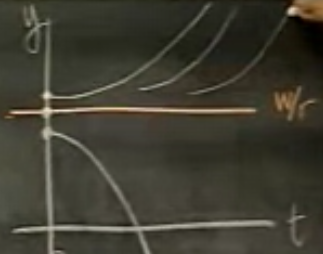
\includegraphics[height=4cm]{5_6.png}

$w/r$ uzerindeki tum baslangic noktalari digerlerinin tercumesi, tasinmis
hali (translations), ustte belirttigimiz gibi. 

Lojistik Denklem

Bu denklem nufus artisini hesaplamak icin kullanilir. 

Nufus $y(t)$.  Temel denklem

\[ \frac{dy}{dt} = ky\]

$k$ buyume hizi

$k$ sabit ise buyumeye basit buyume adi verilir. Lojistik buyume biraz daha
cetrefil bir tur buyumedir. Bu model der ki sabit buyume sekli fazla
temeldir, hicbir canli sinirsiz bir sekilde buyuyemez, kaynaklar buna
musaede etmez. 

Lojistik denkleme gore artma orani (rate) da zaman gore degisir, nufus
arttikca oran azalir. Bu azalisi modellemek icin en basit form $k = a - by$
gibi bir fonksiyondur. Onceki formulun icine koyarsak

\[ \frac{dy}{dt} = ay - by^2 \]

Bu nihai denklem Lojistik Denklemidir, ve nufus artisi haricinde pek cok
kullanim alani vardir. Hastalik yayilmasi, dedikodu (rumor) aktarimi,
buyumesi, vs. gibi.

Denklemi cozmek icin degiskenler ayrilir, ayrica kismi kesirler (partial
fractions) adinda bir teknik lazimdir. Biz cozumu yapmadan denklem hakkinda
bilgi edinmeye ugrasacagiz. 

Kritik noktalar: 

\[ 0 = ay - by^2 \]

\[ y(a-by) = 0\]

\[ y = 0, y=a/b \]

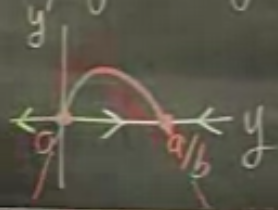
\includegraphics[height=4cm]{5_7.png}

Iki kritik nokta bulduk. Simdi eksenleri $y'$ ve $y$ olan bir grafik
cizelim. Bu grafikte $y'$ nin pozitif mi negatif mi olduguna gore $y$'nin
azalip azalmayacagini oklar ile gosterecegiz. Parabolun altinda $y'$
negatiftir, $y$ buradalarda artar (ok saga dogru), diger yerlerde tam
tersi. 

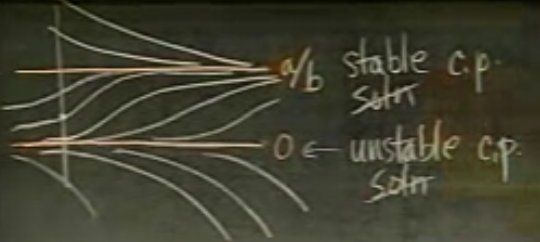
\includegraphics[height=4cm]{5_8.png}

Simdi $y$ ve $t$ grafigi cizelim. Eger baslangic noktasi $a/b$ altindaysa
ve orada artis var ise, ayrica entegral egrilerinin hicbir zaman
birbirleriyle cakisamayacagini soylemistik, o zaman bu artis $a/b$ duz
cizgisine gelip dayanacak ama onu gecmeden ona paralel saga dogru devam
edecektir. Her artis birbirinin saga dogru tercumesidir, cizim bunu tam
gosteremiyor ama asagi yukari o temsil edilmeye ugrasildi.

$a/b$ uzerinde benzer ama tersi bir durum, baslangictan $a/b$'ye azalis
oluyor. $a/b$ noktasina stabil kritik nokta (critical point, hoca
c.p. yazdi) ismi veriliyor, $0$ noktasi stabil olmayan kritik nokta. Hoca
cozum (solution) kelimesinin uzerini cizdi, ama, tabii ki bu noktalarin
ayni zamanda birer cozume de tekabul ettigini soyledi.

Stabiliteyi anlamak icin grafikte kritik noktalara bakilir, oklar eger o
noktadan ``kaciyorsa'' o nokta stabil olmayan, o noktaya dogru
``gidiyorsa'' o nokta stabil nokta demektir.

Ucuncu bir secenek ise su. Eger $y'$ ve $y$ egrisi alttaki gibiyse ne olur?

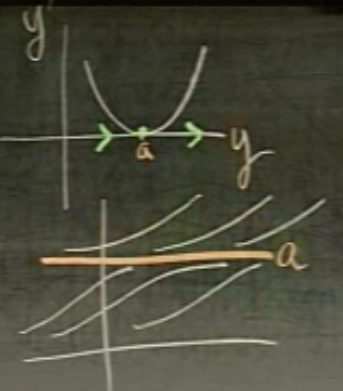
\includegraphics[height=4cm]{5_9.png}

Bu durumda baslangic $y$'si $a$ altinda ise $a$'ya dogru gidilir, ustunde
ise ondan kacilir. Yani stabilite $a$'nin neresinde oldugunuza gore
degisir. Bu tur noktalara bu sebeple ``yari stabil (semi-stable)'' adi
veriliyor. 

Simdi lojistik denklemin degisik bir turune gelelim. 

Hasatla Eksiltilen Lojistik Denklemi

Mesela somon baligi yetistirilen bir balik ciftligi dusunelim. 

Hasat $h$: sabit sayida alinan balik

Yani nufusa oranla degil, belli sabit sayida somonun alinmasindan
bahsediyoruz. Denklem

\[ \frac{dy}{dt} = ay - by^2 - h \]

Dikkat, $hy$ degil, sadece $h$. 

Bunu cozmek icin ne yapardik? Yapilmamasi gereken onu sifira esitleyip
karesel denklem ile bogusmak, koca bir formulu cozmeye ugrasmak, vs. Daha
iyisi, hemen bir grafik cizelim. 

Eger $h=0$ ise, grafik neye benzer? $h$'yi arttirdikca grafik nasil degisir
(asagi iner)? 

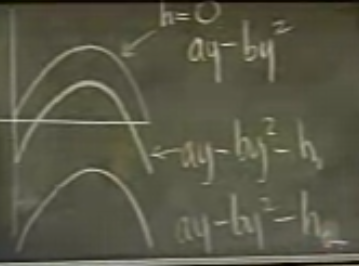
\includegraphics[height=4cm]{5_10.png}

Eger $h=0$ egrisini yatay eksene degecek kadar, bir $h_m$ degeri kadar
asagi indirseydik, 

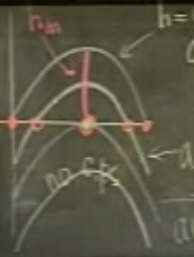
\includegraphics[height=4cm]{5_11.png}

$h_m$ icin $y$ ve $t$ grafigi suna benzer. 

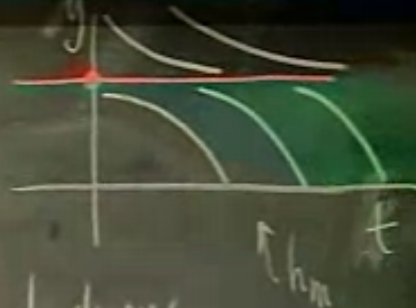
\includegraphics[height=4cm]{5_12.png}

Yani kirmizi cizgi hem altinda hem ustunde inis vardir. $h_m$ noktasinin
model acisindan su anlami vardir: $h_m$ yapilabilecek en fazla hasat
oranini gosterir, o orandan fazla yapilacak hasat zamanla somonlari
tuketecektir. Kirmizi cizgi ustunden basladigimiz ve $h_m$ oranindan fazla
(cok az fazla bile olabilir) bir oranla hasat yaptigimiz takdirde, somonlar
bitmez.



\end{document}










